\begin{pastexam}[label={px:ncku-114-cce-ds-08}]{成大電通所 114 學年度 單選題第 8 題}
（單選；每題 5 分，答錯倒扣 2 分）

Prim algorithm is used to construct a minimum spanning tree $T$ by using the data structure ``set''. They form a
set for all nodes in the beginning and gradually merge two nodes until $T$ is found. Please identify the first
edge which form a cycle in $T$ during the procedure and the number of sets formed at that moment.

\begin{center}
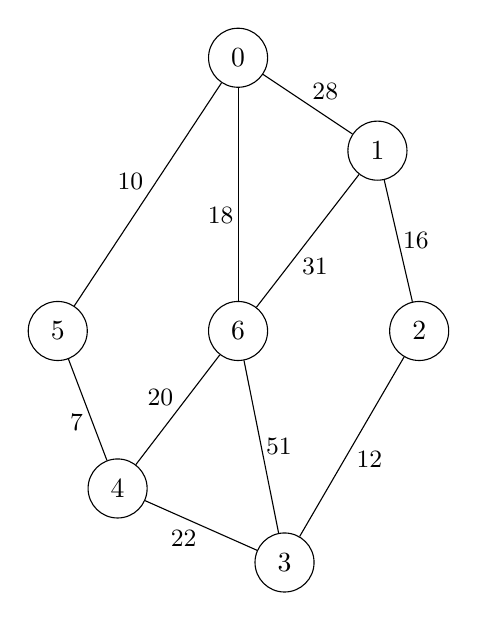
\begin{tikzpicture}[v/.style={circle,draw,inner sep=1pt,minimum size=7.5mm},w/.style={font=\small,inner sep=1.5pt}]
\node[v] (n0) at (3.35,-0.88) {0};
\node[v] (n1) at (5.12,-2.06) {1};
\node[v] (n5) at (1.06,-4.35) {5};
\node[v] (n6) at (3.35,-4.35) {6};
\node[v] (n2) at (5.65,-4.35) {2};
\node[v] (n4) at (1.82,-6.35) {4};
\node[v] (n3) at (3.94,-7.29) {3};
\draw[] (n0) -- node[w,above right] {28} (n1);
\draw[] (n0) -- node[w,above left] {10} (n5);
\draw[] (n0) -- node[w,left,pos=0.6] {18} (n6);
\draw[] (n1) -- node[w,below right,pos=0.6] {31} (n6);
\draw[] (n1) -- node[w,right] {16} (n2);
\draw[] (n5) -- node[w,below left] {7} (n4);
\draw[] (n6) -- node[w,above left] {20} (n4);
\draw[] (n6) -- node[w,right] {51} (n3);
\draw[] (n2) -- node[w,below right] {12} (n3);
\draw[] (n4) -- node[w,below left] {22} (n3);
\end{tikzpicture}
\end{center}
a) edge (3, 6) and 2 set\quad b) edge (4, 6) and 4 set\\
c) edge (0, 1) and 3 set\quad d) edge (4, 6) and 3 set\\
e) None of the above
\end{pastexam}

\begin{pastsoln}
答案：b) edge (4, 6) and 4 set。

\textbf{解讀}。 題目說用 Prim 演算法，又說「一開始每個節點各自一個集合，逐步把兩個合併」。 這裡的讀法是：每個頂點一開始自成
一個集合，Prim 每把一個頂點拉進樹，就把它的集合併進樹的集合；「形成環的邊」是兩端已經在同一個集合（都在樹上）、
被丟掉的邊。 題目沒說從哪個頂點開始，照慣例從 0 開始。 Prim 每一步取「一端在樹上、一端不在」的最小邊，用資結書
虛擬碼~24.4 那種把邊放進優先佇列、取出時才檢查的寫法，就會取出兩端都已在樹上的邊，那就是本題要的「第一條成環的邊」。

邊（權重）：$(5,4)$ 7、$(0,5)$ 10、$(2,3)$ 12、$(1,2)$ 16、$(0,6)$ 18、$(4,6)$ 20、$(3,4)$ 22、$(0,1)$ 28、$(1,6)$ 31、
$(3,6)$ 51。
\begin{center}
\small
\begin{tabular}{llll}
\toprule
步驟 & 取出的邊 & 結果 & 集合 \\
\midrule
開始 & & 樹 $\{0\}$ & $\{0\},\{1\},\{2\},\{3\},\{4\},\{5\},\{6\}$（7 個） \\
1 & $(0,5)$ 10 & 5 加入 & $\{0,5\},\{1\},\{2\},\{3\},\{4\},\{6\}$（6 個） \\
2 & $(5,4)$ 7 & 4 加入 & $\{0,4,5\},\{1\},\{2\},\{3\},\{6\}$（5 個） \\
3 & $(0,6)$ 18 & 6 加入 & $\{0,4,5,6\},\{1\},\{2\},\{3\}$（4 個） \\
4 & $(4,6)$ 20 & 4、6 都已在樹上，成環，丟掉 & 仍是 4 個 \\
\bottomrule
\end{tabular}
\end{center}
第 1 步時樹只有 0，可選的是 $(0,5)$ 10、$(0,6)$ 18、$(0,1)$ 28，取 10。 第 2 步多了 5 的邊 $(5,4)$ 7，取 7。 第 3 步
候選是 $(0,6)$ 18、$(4,6)$ 20、$(4,3)$ 22、$(0,1)$ 28，取 18。 第 4 步最小的是 $(4,6)$ 20，但 6 已經在樹上，加了會和
$4\text{--}5\text{--}0\text{--}6$ 形成環。 這時有 4 個集合，選 b)。 之後依序加入 $(4,3)$ 22、$(3,2)$ 12、$(2,1)$ 16，
最小生成樹的總權重 $10 + 7 + 18 + 22 + 12 + 16 = 85$。

\textbf{其他選項}：a) $(3,6)$ 是權重最大的邊，不會是第一條；c) $(0,1)$ 28 在 $(4,6)$ 之後才會被考慮；d) 邊對了，集合數錯。
附帶一提，題目描述的「每點一個集合、逐步合併」其實是 Kruskal 的做法（資結書第~24.2~節）。 照 Kruskal 依權重由小到大
處理：7、10、12、16、18 都接受，集合從 7 個合併到 2 個（$\{0,4,5,6\}$、$\{1,2,3\}$），接著 $(4,6)$ 20 成環，第一條成環的邊
同樣是 $(4,6)$，但那時是 2 個集合，不在選項裡。 題目明說 Prim，所以答 b)。
\end{pastsoln}
